\documentclass[titlepage,12pt,a4paper]{article}

\usepackage[pdftex]{graphicx}
%\usepackage[symbol]{footmisc}
\usepackage[utf8]{inputenc}

\usepackage{tikz}
\usetikzlibrary{shapes,decorations}

\usepackage{makeidx}
%\usepackage{showidx}
\usepackage{parskip}
\usepackage{float}
\usepackage{calc}
\usepackage{pdfpages}
\usepackage{todonotes}
\usepackage{amsfonts}
\usepackage{amsmath}
\usepackage{pifont}
\usepackage{pdflscape}
\usepackage{geometry}
\usepackage{listings}

\usepackage[backref=page]{hyperref}
\def\backref#1{{\scriptsize [#1]}}

\newcommand{\HRule}{\rule{\linewidth}{0.35mm}}

\def\theaipage{\string\hyperpage{\thepage}}

\hypersetup{
    %bookmarks=true,         % show bookmarks bar?
    unicode=false,          % non-Latin characters in Acrobats bookmarks
    pdftoolbar=true,        % show Acrobats toolbar?
    pdfmenubar=true,        % show Acrobats menu?T
    pdffitwindow=false,     % window fit to page when opened
    pdfstartview={FitH},    % fits the width of the page to the window
    pdftitle={Design of Liaison System, TFE4140 Term Project},    % title
    pdfauthor={Stian Hvatum, Benjamin Bjørnseth},     % author
    pdfsubject={TFE4140 Term Project},   % subject of the document
    pdfcreator={Stian Hvatum, Benjamin Bjørnseth},   % creator of the document
    pdfproducer={Stian Hvatum, Benjamin Bjørnseth}, % producer of the document
    pdfnewwindow=true,      % links in new window
    colorlinks,       % false: boxed links; true: colored links
    linkcolor=black,          % color of internal links
    citecolor=green,        % color of links to bibliography
    filecolor=magenta,      % color of file links
    urlcolor=cyan           % color of external links
}

\begin{document}

\begin{titlepage}

\begin{center}

    %    \includegraphics[scale=0.7]{./figures/Fortitudo_floris}\\[1cm]

\textsc{\LARGE TTK4850 - EiT Byggelandsbyen}\\[0.2cm]

\HRule \\[0.5cm]

{\huge Miksebord}\\[0.2cm]
\small{Project report}\\[1cm]

\begin{table}[h]
\centering
\begin{tabular}{rl}
Thomas Hasfjord   &  Bård Bakken Stovner\\
Andreas Eilertsen & Håkon Furre Amundsen\\
\multicolumn{2}{c}{Stian Hvatum}
\end{tabular}
\end{table}

\vfill
\large{\today}

\end{center}

\end{titlepage}

\pagenumbering{Roman}
\abstract This report contains our solution to the term project in the
course TFE4140. We describe our design of a liaison system implemented
on an FPGA, meant to perform a majority vote amongst microcontrollers
transmitting data words serially. The main focus of our implementation
was to keep the area usage as low as possible, measured in the number
of LUTs used on the FPGA. We discuss alternative solutions, and
examine their relative strenghts and weaknesses.  Our proposed
solution uses 32 LUTs, and runs with a clock frequency of 318.715 MHz.

\newpage
\tableofcontents
\newpage
\listoffigures
\listoftables

\newpage
\pagenumbering{arabic}
%sections goes here, use \input{file[.tex]}

\section{Introduction}
\section{Description of problem}
\section{Description of solution}

\newpage
\section{Design}
\begin{figure}[h]
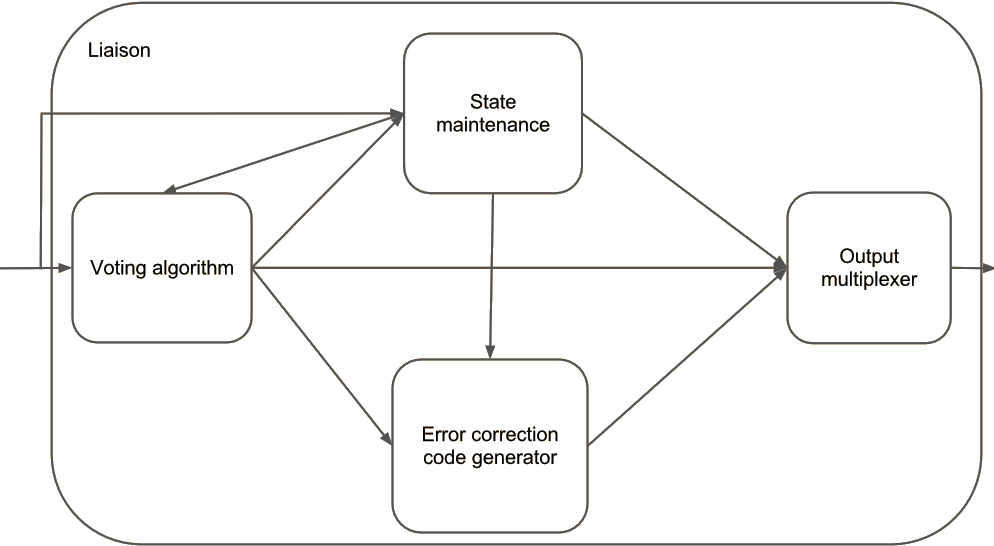
\includegraphics[width=15cm]{design/fig_overview}
\caption{Modules overview}
\label{fig:overview}
\end{figure}

An overview of our system design is depicted in
\autoref{fig:overview}. Conceptually, the internals of the Liaison can
be modeled as four different components, each responsible for a
certain task as indicated by their respective names.

\subsection{System Assumptions}
There are certain elements of the system behaviour and environment
that is not specified in the requirements. We have therefore done some
assumptions for our implementation.

\begin{itemize}
\item Outside of periods in which the microprocessors are supposed to
  be sending data to the Liaison\footnote{before or more than 8
    cycles after a {\ttfamily di\_ready} signal}, we assume that the
  microcontrollers are not necessarily driving the lines, and thus we
  cannot tag the microcontrollers.

\item We have assumed that two failing microcontrollers within the
  same clock cycle should not happen. This assumption is made since it
  is, in general, not possible to detect the simultaneous failure of
  two or more microcontrollers. For instance, if three controllers are
  left, and two of them fail and produce the wrong output, they will
  be assumed to be working while the microcontroller that is actually
  producing correct results will be tagged as erroneous. Since there
  is no other distinction between the microcontrollers than the data
  they produce, it will be impossible to detect a difference between
  this situation and one in which one microcontroller fails. If four
  microcontrollers are working, and two fails, the system logic will
  select two controllers for failure without knowing which really has
  failed. If the selection was correct, the system will continue
  functioning; if not, the two failed microcontrollers that was left
  as working will most likely shortly provide inconsitent data, and
  the system will be considered broken.

\item The requirements do not specify what data should be output when
  the system is failing. We assume that since the receiver will know
  that the system is broken, the data sequence can be whatever it
  likes. The most easy solution is therefore to output whatever the
  combinatorial circuits responsible for the voted data output, and we
  have not created any special logic to adjust the data message.

\end{itemize}


\subsection{Voting algorithm}
\label{sec:votingalgorithm}
The system needs to distinguish between the working and the
malfunctioning microcontrollers. To do this, the voting module knows
what microcontrollers that has shown sign of failure from earlier
voting, and it needs to vote for the majority result of working
microcontrollers. This modules receives input directly from the
microcontrollers, and it gets the current system state from the State
Maintainance module.

The algorithm in our design works by partitioning the microcontrollers
into two pairs. For the following explanation, the microcontrollers
will be labeled A, B, C and D, and the groups in the partition will be
labeled (A, B) and (C, D).

First, each group performs what will be referred to as a local
vote. The result from this local vote is tabulated in
\autoref{tab:localvote}.

\begin{table}[htbp]
  \centering
  \caption{Local vote between microcontroller pairs}
  \begin{tabular}{|c|c|}
    \hline
    \textbf{Condition} & \textbf{Result} \\ \hline
    MCU1 and MCU2 both untagged & MCU1 data $\wedge$ MCU2-data \\ \hline
    Only MCU1 untagged & MCU1 data \\ \hline
    Only MCU2 untagged & MCU2 data \\ \hline
    Both tagged   & 0 \\ \hline
  \end{tabular}
  \label{tab:localvote}
\end{table}

The local vote gives the majority vote between the two
microcontrollers. In the case of a tie, or both microcontrollers being
tagged as erroneous, the output from the vote is 0. 

The algorithm then proceeds by distinguishing between three different
scenarios. These scenarios are tabulated in
\autoref{tab:globalvote}. The condition in each row also implies that
none of the conditions in rows above it hold.

\begin{table}[htbp]
  \centering
  \caption{Final vote result}
  \begin{tabular}{|p{7cm}|c|}
    \hline
    \textbf{Condition} & \textbf{Result} \\ \hline
    A, B untagged and (A,B)-result is not a tie & (A,~B)-result \\ \hline
    Data from C and D is equal & (C,~D)-result \\ \hline
    Neither pair is safe  & (A,~B)-result $\vee$ (C,~D)-result \\ \hline
  \end{tabular}
  \label{tab:globalvote}
\end{table}

First, it checks whether both A and B are untagged and have the same
data value. If this is the case, then the output from the local vote
of (A,~B) will have two votes, which is enough to ensure either
majority or a tie no matter what the result from (C,~D) is.

If this is not the case, then either A or B is faulty, and the (A,
B)-result represents at most one vote. If the data from
microcontroller C and D is the same, then it represents two, one or
zero votes to the (C,~D)-result without providing any votes which
could strengthen the (A,~B)-result.

\begin{itemize}
\item If the (C,~D)-result represents two votes, it is the majority
  result, since the (A,~B) group can oppose it with at most one vote. 
  
\item If the (C,~D)-result represents one vote
  \begin{itemize}
  \item If the (A,~B)-result is a tie, then the (C,~D)-result will be
    the decisive vote. 
  \item If the (A,~B)-result represents one vote, then the (C,
    D)-result is either the majority result or there is a tie. In
    either case, the (C,~D)-result is a valid result from the vote.
  \item If the (C,~D)-result represents zero votes, then the system is
  \end{itemize}

\item If the (C,~D)-result represents zero votes, then the system must
  be broken since the (A,~B) result only represents at most one vote
  and as such only one microcontroller is still functioning correctly.
\end{itemize}

If the data from C and D is not the same, then neither pair of
microcontroller is guaranteed to represent the majority on its
own. The remaining possibilities are as follows

\begin{itemize}
\item If the (A,~B)-result is a tie, then its value is zero. It is
  thus safe to output this value ORed with the (C,~D)-result, which is
  the decisive vote.

\item If the (A,~B)-result represents a single vote
  \begin{itemize}
  \item If the (C,~D)-result is a tie, then by the same reason as in
    the first point (A,~B)-result $\vee$ (C,~D)-result is a valid
    voting result.

  \item If the (C,~D)-result also represents a single vote
    \begin{itemize}
    \item If the (A,~B)-result equals the (C,~D)-result, (A,~B)-result
      $\vee$ (C,~D)-result will produce this value.
    \item If the results are not equal, the vote is a tie and the
      output can be anything.
    \end{itemize}
  \end{itemize}

\item Any other condition represents a system broken state, in which
  only one or zero microcontrollers are still working. For these
  scenarios, the result from the vote does not matter.

\end{itemize}

\subsection{State maintainance}
The State Maintainance module is responsible for all internal states
of the system. The system keeps track of what microcontrollers that
can no longer be trusted. This works by tagging those microcontrollers
were the signal differs from the voted signal from the Voter
module. When a microcontroller has been tagged, the tag is not cleared
until the entire system is reset.

This module also outputs a system status vector as part of the Liaison
output. This vector has one of four states as shown in
\autoref{tab:systemstatus}.  The output status is a direct mapping
from the internal tag-vector, and works simply as a lookup table.

At last, the State Maintainance module is also responsible for
counting what output is sent at each clock tick. Since we are
outputing a serial data stream where different sections of the stream
have different sources (data, status, ECC), we need to keep track of
the position of the current data bit.



\subsection{Error Correcting Code Generator}
To provide reliable output for long distance transmission of data, the
Liaison System was required to add an error correcting code (ECC) to
its data packets. As stated in \autoref{sec:problem}, the ECC should
be able to correct one bit errors and detect two bit errors. To
fulfill the first criteria, we use a (15, 11)
Hamming-code\cite{ecc}. Since the Liaison sends eleven data bits ---
eight for the voted data and three for the status --- using four
parity bits is sufficient to provide detection and correction for one
bit errors. To be able to detect two bit errors, one can use an extra
parity bit covering all the transmitted bits, including data, status
and the four other ECC bits. This final parity bit is called
SECDED-bit, since it makes the Hamming code a Single Error Correction
Double Error Detection code\cite{ecc}. For simlicity, we will refer to
this error correction code scheme as a (16, 11) Hamming code. The
calculation of the parity bit is shown in \autoref{tab:hammingcode},
showing which data bits are covered by each parity bit.

\begin{table}[htbp]
  \centering
  \caption{Hamming Code Data Bit Coverage}
  \begin{tabular}{|c|c|c|c|c|c|c|c|c|c|c|c|c|c|c|c|c|}
    \hline
   & d0 & d1 & d2 & d3 & d4 & d5 & d6 & d7 & d8 & d9 & d10 & p0 & p1 & p2 & p3 & p4 \\ \hline
p0 & X  & X  &    & X  & X  &    & X  &    & X  &    & X   & X  &    &    &    &    \\ \hline
p1 & X  &    & X  & X  &    & X  & X  &    &    & X  & X   &    & X  &    &    &    \\ \hline
p2 &    & X  & X  & X  &    &    &    & X  & X  & X  & X   &    &    & X  &    &    \\ \hline
p3 &    &    &    &    & X  & X  & X  & X  & X  & X  & X   &    &    &    & X  &    \\ \hline
p4 & X  & X  & X  & X  & X  & X  & X  & X  & X  & X  & X   & X  & X  & X  & X  & X  \\ \hline
    
  \end{tabular}
  \label{tab:hammingcode}
\end{table}


The Error Correcting Code Generator generates (16,11) Hamming code on
the fly and attaches the code at the end of the output stream. This
module uses information from the Voter to get the first eight data
bits and information from the State Maintainance to get the status
word. It also uses information of current data bit position from the
State Maintainance module, since Hamming Code is generated using
parity of bits at specific positions\cite{ecc}.

\subsection{Output Multiplexer}
Since the Liaison System needs to send output from each of the three other modules at specific clock cycles when specific events has occured, we need
a logic piece of hardware that can multiplex all modules and allways output the correct signal. The Output Multiplexer uses the position of current data bit
from the State Maintainance module to select what module to send data from.

\newpage
\section{Implementation}

\begin{figure}
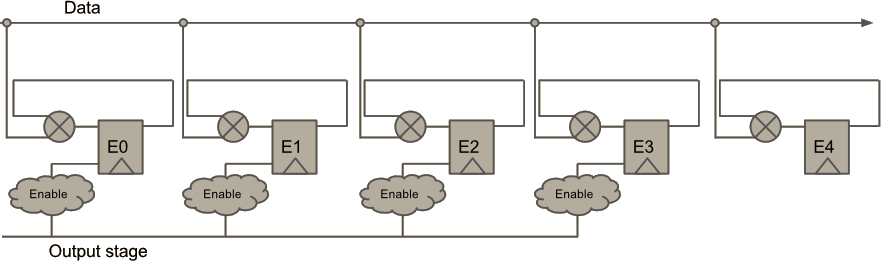
\includegraphics[width=15cm]{implementation/fig_ecc}
\caption{Implementation of Hamming(16,11)}
\label{fig:ecc}
\end{figure}

\newpage
\section{Verification}
\subsection{Overview}
The liaison system was verified utilizing automated testbenches. The testbenches uses VHDL assertions to notify the author if any
of the tests failed. In order to create a good and short but extensive testbench, we have built a collection of procedures that takes input, expected output
and expected system status after all input has been sent.

The test cases was divided into three blocks.
\begin{itemize}
\item The first test block consists of 8 tests that asserts the normal behaviour. It is done with some easy cases and a 2 cycle delay between inputs.

\item The second test block consists of 24 cases that at some point broke our logic.  tests where our design was likly to have flaws. During development, these tests were
triggered often, proving their value.

\item The third and last test block is a permutation of working state and all 4! fail states, each with all MCUs sending
all possible inputs (all MCUs sends the same value to keep the number of tests down to an affordable number). This block consists of 269 376 different test cases,
and cover almost any possible state. The states that are not covered are those where one of the MCUs fails in the middle of the transaction, which are covered in
the second block.
\end{itemize}

Since all permutations of fail states and all permutations of valid input within these states
were applied to the circuit during simulation, we are confident that the Liaison System is working correctly. We have also tested the circuit with a post-place and route
simulation verifying that the output is also correct with timing taken into account\footnote{The timing simulation was done with iSim from Xilinx, synthesised with XST. Both tools are part of the ISE Design Suite}.

\subsection{Conformance with requirements specification}
This section explain the conformance with each point in the system requirements specification.
\begin{enumerate}
\item{\textbf{The Liaison Interface}} \hfill\\
    Our implementation of the Liaison System follows the signaling interface given by the requirements\cite{task}.

\item{\textbf{Voting}} \hfill\\
    The Voting algorithm has been tested and confirmed to be working. This was done by enumerating all
    permutations of input and state, and then check the Voters result against expected output using
    VHDL assertions.

\item{\textbf{Error tagging}} \hfill\\
    The error tagging is not specified in the requirements, but is nessesary in our implementation to
    achieve correct System Status bits and correct Voting. The error tagging was tested with the same
    tests as the Voting algorithm and does conform with the expected behaviour.

\item{\textbf{System status}} \hfill\\
    The System Status is needed to tell the receiver about the wellness of the microcontrollers. Since
    there exists a direct mapping between the Error tagging and the System Status, this is also
    included in the same tests as Error tagging and Voting.

\item{\textbf{Error correcting code}} \hfill\\
    The Error correcting code is a specific part of the requirements\cite{task}. The module was tested by writing
    a testbench function that generates (15,11)-Hamming Code with SECDED from an 11-bit word. This
    procedure was added to the enumerated tests from the Voter-test such that for each input, the testbench
    would automatically expect a specific ECC. If the ECC from the function was not equal to the output
    of the Liaison, assertions were raised to the tester. Since the soft function agrees with the simulated
    hardware, we are certain that the ECC-module works as specified in the requirements. The ECC-generating
    software function can be found in \autoref{apx:ecc}.

\item{\textbf{Reset behaviour}} \hfill\\
    On reset, The Liaison is set back to inital state on next clock cycle. The reset is stricly synchronous,
    as stated in the requirements\cite{task}, and is thus only read on rising edge of the clock. We have
    tested that reset works for any final state when a data sequence finished, but we have not tested the
    behavoiur of a reset in the middle of a transmission. By simple code inspection, we see that the
    reset is not aware of current system status, but simply sets all the state variables back to initial
    state. That means that after a reset signal is asserted along with rising edge of the clock, the system
    will not process data until a new {\ttfamily di\_ready}.

\item{\textbf{System consitency}} \hfill\\
    Since all possible inputs for both the Voter and the ECC module has been exhaustively tested, and 
    Since very little of the internal system logic is dependent on both system status and current bit-position,
    we are sure that the exhaustive tests run on the Voter and the ECC module is sufficient to conclude that 
    the entire system is consitent with the requirements. All enumerations of fail states have been tested, all combinations
    of input to the ECC module have been tested, and the Output Multiplexer cares only about current output bit position,
    and is thus also exhaustivly tested.

\item{\textbf{New data after $11+m$ cycles}} \hfill\\
    Most of the test cases send data directly after previous data word was correctly received, so 
    Our implementation of the Liaison System follows the signaling interface given by the requirements.

\end{enumerate}

\todo{Include timing diagrams}
\newpage
\section{Conclusion}
\section{Conclusion}
From testing and verifying software prototype this report displays a working proof of concept of a feedback cancellation  algorithm based on the two-stage NHS method. The front end interface and output interface has been constructed and tested. All has been verified to work according to specifications.

\section{Further work}
The NHS algorithm is a simple one, and in this design it is further simplified. There are a number of ratios used in NHS that can be calculated to improve the detection capabilities, examples of these ratios can be found in \cite{van_waterschoot_fifty_2011}. \\

There are also more advanced algorithms for removing feedback, for instance a AFC-method(Adaptive Feedback Cancellation). The AFC uses system identification to detect the feedback path and models its inverse, thereby cancelling the coupling. Details can be found in \cite{van_waterschoot_fifty_2011}.\\

Transforming the system from a software prototype to a hardware prototype can be done by as previously stated using a FPGA as the DSP-module and implementing the algorithm on it.\\
The broader goal is a finished product. Working on product design, a complete hardware design and doing marked research are all important tasks in completing the project.
\newpage

\appendix
\bibliographystyle{plain}
\bibliography{bibliography}

\end{document}
